\chapter{Fonctionnalités de CaWaQS-Viz}
\label{chap-features}

\renewcommand{\headrulewidth}{0.3pt}
\fancyhead[LE]{\thepage} \fancyhead[RE]{\nouppercase{\textbf{\leftmark}}}
\fancyhead[RO]{\thepage} \fancyhead[LO]{\nouppercase{\textbf{\rightmark}}}
\fancyfoot[L,C,R]{}

\setlength{\parindent}{0.35cm}

\minitoc
\newpage

% ================================================================
\section{\gui{Calibration Tools} : outils de calage}
\label{sec-calib-tools}

La boîte de dialogue \gui{Calibration Tools} (\cref{fig_DialogCalibrationTools}) propose des outils utiles pour caler un nouveau modèle \cawaqs. Ces fonctionnalités ne sont pas toutes opérationnelles à ce jour. En effet, la majorité d'entre elles n'a pas été prise en compte lors de la refonte du T1 2026. Elles restent néanmoins déjà présentes dans le code. Une restructuration et un raccordement minimes suffiraient à les rendre à nouveau opérationnelles. \alertwarning{Toutes les fonctionnalités non encore opérationnelles sont signalées dans le guide utilisateur par l'acronyme WIP (Work in Progress) ou par un symbole /!\textbackslash{} dans QGIS.}

\begin{itemize}
    \item  \gui{Modify a parametrisation file} (\cref{sec-feat-modify-param}) - WIP : outil de modification des fichiers de paramétrisation des différents compartiments modélisés ;

    \item  \gui{Statistical Criteria} (\cref{sec-critstat}) : outil de calcul des critères de performance du calage du modèle ;

    \item \gui{Run-off coefficient calculation} (\cref{sec-runoff-coef}) WIP : outil de calcul des coefficients de ruissellement simulés ;

    \item   \gui{Compare sim/obs} (\cref{sec-com-simobs}) WIP : outil de visualisation des chroniques simulées et observées.
\end{itemize}

\begin{figure}[H]
    \centering
    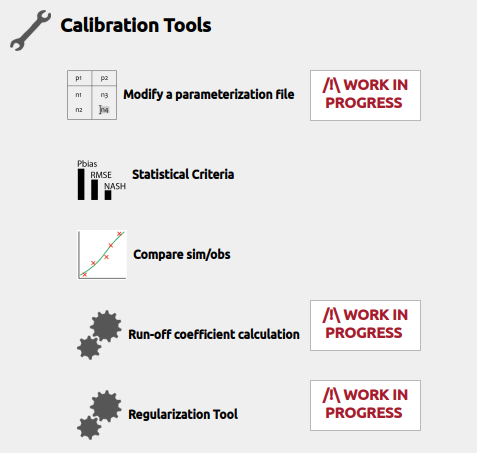
\includegraphics[width=0.65\linewidth]{
        2_application_user_guide/fig/DialogCalibrationTools.png
    }
    \caption{Boîte de dialogue des outils de calage.}
    \label{fig_DialogCalibrationTools}
\end{figure}

\subsection{WIP : modification des fichiers de paramétrisation}
\label{sec-feat-modify-param}

Les fichiers de paramétrisation peuvent être modifiés depuis la boîte de dialogue \gui{Modifying a parametrization file} (\cref{fig-dialog_modif_param_file}). La résolution dépendra du fichier de calage à sélectionner dans le menu déroulant. La table peut être affichée en cliquant sur 
\includegraphics[height=0.45cm]{2_application_user_guide/fig/show.png}.\\

Si la table attributaire affichée ne contient pas les champs du fichier de paramétrisation, la résolution peut être liée à son fichier de paramétrisation dans la boîte de dialogue \gui{Link resolution to its parameterisation file}, accessible en cliquant sur 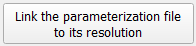
\includegraphics[height=0.55cm]{
    2_application_user_guide/fig/AccesDialogLinkParamResolution.png
}. L'utilisation de cette boîte de dialogue est décrite en \cref{sec-link_table}.

\begin{figure}[H]
    \centering
    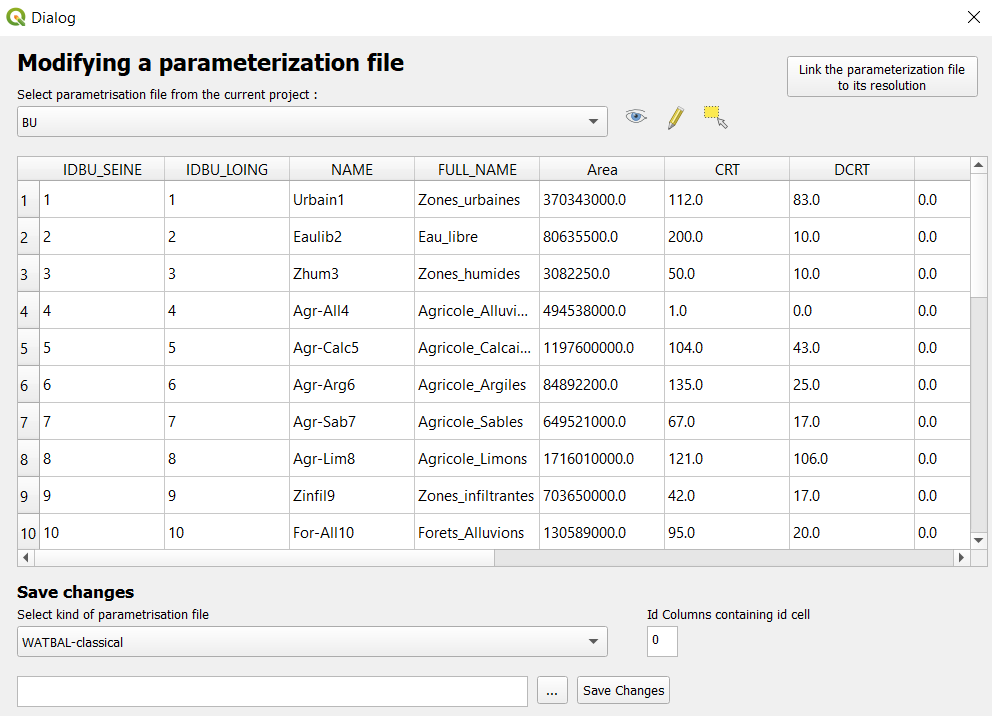
\includegraphics[width=1\linewidth]{
        2_application_user_guide/fig/DialogModifParamFile.png
    }
    \caption{Boîte de dialogue de modification des fichiers de paramétrisation.}
    \label{fig-dialog_modif_param_file}
\end{figure}

Une fois les paramètres modifiés dans la table affichée, celle-ci peut être enregistrée. Le nouveau chemin du fichier peut être spécifié en sélectionnant 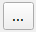
\includegraphics[height=0.45cm]{2_application_user_guide/fig/SelectPath.png}. Précisez l'identifiant de la colonne contenant l'identifiant ou le nom de la maille\footnote{ATTENTION : pour rappel, les identifiants de colonnes commencent à \textbf{0}.}.

\subsection{WIP : lier une table attributaire à sa résolution}
\label{sec-link_table}

Les paramètres du fichier de paramétrisation seront directement importés comme champs dans la table attributaire du fichier de résolution concerné. Pour créer ce lien, il faut choisir un type de fichier de paramétrisation (selon le compartiment et le type de fichier de paramétrisation), la résolution \cawaqs, et le chemin vers ce fichier de paramétrisation. Différents types de fichiers de paramétrisation existent et sont listés dans la table \ref{tab-type_param_file}.

\begin{figure}
    \centering
    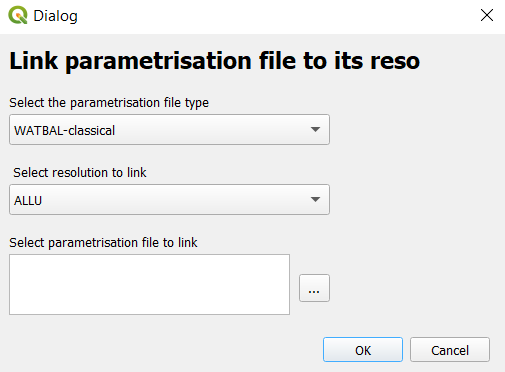
\includegraphics[width=0.7\linewidth]{
        2_application_user_guide/fig/DialogLinkTable.png
    }
    \caption{Boîte de dialogue de liaison d'une table attributaire à sa résolution.}
    \label{fig:enter-label}
\end{figure}

\begin{table}[H]
    \centering
    \begin{tabular}{m{4cm}|m{4cm}|m{4cm}}
        \hline
        \textbf{Compartiment} & \textbf{Type de fichier de paramétrisation} & \textbf{Paramètres listés dans la table}             \\
        \hline
        \script{WATBAL}       & Classique                                   & CRT, DCRT, R, FN, CQR, CQRMAX, CQI, CQIMAX et RNAP       \\
        \hline
        \script{WATBAL}       & Excès d'infiltration                        & CRT, DCRT, R, FN, CQR, CQRMAX, CQI, CQIMAX, RNAP et RINF \\
        \hline
        \script{AQ}           & Transmissivité                              & T                                                        \\
        \hline
        \script{AQ}           & Emmagasinement (coefficient d'emmagasinement) & S                                                      \\
        \hline
        \script{AQ}           & Conductance                                 & C                                                        \\
        \hline
    \end{tabular}
    \caption{Fichiers de paramétrisation pris en charge par \texttt{\cwv}.}
    \label{tab-type_param_file}
\end{table}

\subsection{\script{Statistical Criteria} : calcul des critères de performance statistique aux points d'observation}
\label{sec-critstat}

La boîte de dialogue \gui{Statistical Criteria} (\cref{fig-dialogstatisticalcriteria}) renvoie une couche SIG suivant les géométries de la résolution d'observation propre à la variable analysée. Chaque champ correspond à un critère statistique donné. Les critères statistiques sélectionnés sont calculés sur la période spécifiée dans la section \gui{Period for calculating statistical criteria}.\\

\subsubsection{Critères statistiques calculés par la boîte de dialogue \gui{Statistical criteria}}

\textbf{\gui{Pbias} : biais [$\%$]}
\begin{equation*}
PBIAS = \frac{\sum(\hat{y}_i -y_i)}{\sum y_i} . 100
\quad \quad
\begin{array}{rl}

      y_i & : \text{variable simulée au temps $i$}\\
      O_i & : \text{variable observée au temps $i$}\\
\end{array}
\end{equation*}

\textbf{\gui{Average SIM/OBS}}
\begin{equation*}
    A = \overline{\hat{y}} - \overline{y}
    \quad\quad
    \begin{array}{cc}
         \overline{\hat{y}} :& \text{moyenne des variables simulées} \\
         \overline{y} : & \text{moyenne des variables observées}
    \end{array}
\end{equation*}

\textbf{\gui{Nash} : efficience de Nash-Sutcliffe} \citep{nash1970}
\begin{equation*}
    NSE = 1 - \frac{\sum_{i=1}^n (y_i - \hat{y}_i)^2}{\sum_{i=1}^n (y_i - \overline{y})^2}
    \quad \quad
    \begin{array}{ll}
         y_i :& \text{variable réelle au temps } i \\
        \hat{y}_i :& \text{variable prédite au temps } i \\
    \end{array}
\end{equation*}

\textbf{\gui{RMSE} - erreur quadratique moyenne}
\begin{equation*}
RMSE = \sqrt{\frac{1}{n} \sum_{i=1}^{n} (y_i - \hat{y}_i)^2}
\quad \text{où} \quad
\begin{array}{ll}
    n :& \text{nombre total de jours de simulation} \\
    y_i :& \text{variable réelle au temps } i \\
    \hat{y}_i :& \text{variable prédite au temps } i \\
\end{array}
\end{equation*}

\textbf{\gui{KGE} - efficience de Kling-Gupta} \citep{gupta2012}
\begin{equation}
    KGE = 1 - \sqrt{(r - 1)^2 + (\alpha - 1)^2 + (\beta - 1)^2}
    \quad \quad
    \begin{array}{ll}
         r & : \text{coefficient de corrélation de Pearson} \\
         & \text{entre les séries de variables simulées} \\
         & \text{et observées} \\
        \alpha & : \text{rapport des écarts-types simulé et observé} \\
        \beta  & : \text{biais moyen entre séries simulée et observée}
    \end{array}
\end{equation}




Les critères suivants sont calculés automatiquement : $\overline{y}$, $\overline{\hat{y}}$, $\frac{\overline{\hat{y}}}{\overline{y}}$, $\sigma y$,  $\sigma \hat{y}$, $\frac{\sigma \hat{y}}{\sigma y}$.

\subsubsection{Sortie de la boîte de dialogue \gui{Statistical Criteria}}
\label{sec_stats_crits}

La boîte de dialogue génère des critères statistiques :
\begin{itemize}
    \item aux points d'observation,
    \item à l'échelle de la couche aquifère dans le cas d'une simulation avec compartiment aquifère ;
    \item à l'échelle de l'hydrosystème dans le cas d'une simulation avec compartiment aquifère.
\end{itemize}
\vspace{0.3cm}

\underline{\textbf{Critères statistiques calculés aux points d'observation}}\\
La boîte de dialogue génère la table des critères statistiques aux points d'observation aux formats \script{shapefile} et \script{texte}. Le shapefile est directement intégré au projet \script{QGIS} courant, tandis que le fichier texte se trouvera dans le répertoire \script{../PostProcessing/STATS\_CRITS}. Les critères en sortie sont contenus dans les champs de chaque point de mesure sous les noms définis dans la table \ref{tab_statistical_criteria_crits_fields}.

\vspace{0.2cm}
\underline{\textbf{Critères statistiques calculés à l'échelle des unités aquifères}}\\
Dans le cas d'un calcul des critères statistiques sur le compartiment aquifère, un fichier \script{texte} est enregistré dans le répertoire \gui{Post-Processing} sous \script{../PostProcessing/STATS\_CRITS/AQ\_crits\_xxxx\_xxxx.txt}. Ce fichier liste les critères statistiques de la table \ref{tab_statistical_criteria_crits_fields} définis à l'échelle de chaque unité aquifère.

\vspace{0.2cm}
\underline{\textbf{Critères statistiques calculés à l'échelle de l'hydrosystème}} \\
Des critères statistiques sont définis à l'échelle de l'hydrosystème pour la charge hydraulique souterraine. Ces critères sont écrits dans le fichier \script{../PostProcessing/STATS\_CRITS/AQ\_crits\_xxxx\_xxxx.txt}.\\

\alertwarning{Toutes les sorties shapefile générées par \cwv~sont temporaires. Si elles ne sont pas enregistrées, elles ne seront plus accessibles à la réouverture du projet.}


\begin{table}[H]
    \centering
    \renewcommand{\arraystretch}{1.2}
    \resizebox{\textwidth}{!}{
        \begin{tabular}{rl}
        \hline
        \textbf{Nom du champ de la table de sortie} &  \textbf{Critère statistique} \\
        \hline
        \gui{NObs} & Nombre d'observations sur la période sélectionnée \\
        \gui{AObs} & Moyenne des variables observées \\
        \gui{ASIM} & Moyenne des variables simulées \\
        \gui{SUM\_RATIO} & Rapport de la somme des variables simulées à la somme des variables observées \\
        \gui{StdObs} & Écart-type des variables observées \\
        \gui{StdSim} & Écart-type des variables simulées \\
        \gui{STD\_RATION} & Rapport des écarts-types des variables observées et simulées \\
        \gui{PBAIS} & Biais [\%] \\
        \gui{AVERAGE\ SIM/OBS} & Rapport moyen entre variables simulées et observées \\
        \gui{KGE} & Efficience de Kling-Gupta \\
        \gui{NASH} & Efficience de Nash-Sutcliffe \\
        \gui{RMSE} & Erreur quadratique moyenne \\
        \hline
        \end{tabular}
    }
    \caption{Noms des champs des tables de sortie pour chaque critère statistique}
    \label{tab_statistical_criteria_crits_fields}
\end{table}


\begin{figure}[H]
    \centering
    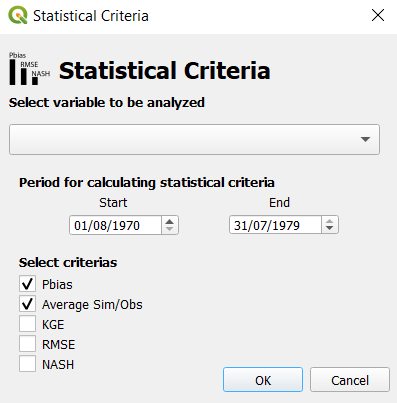
\includegraphics[width=0.5\linewidth]{
        2_application_user_guide/fig/DialogStatisticalCriteria.png
    }
    \caption{Boîte de dialogue \gui{Statistical Criteria}.}
    \label{fig-dialogstatisticalcriteria}
\end{figure}


\subsection{WIP \script{Run-off coefficient calculation} : calcul du coefficient de ruissellement aux stations de mesure de débit}
\label{sec-runoff-coef}

Cette boîte de dialogue calcule le coefficient de ruissellement simulé et observé aux stations de mesure de débit.\\

\begin{figure}[H]
    \centering
    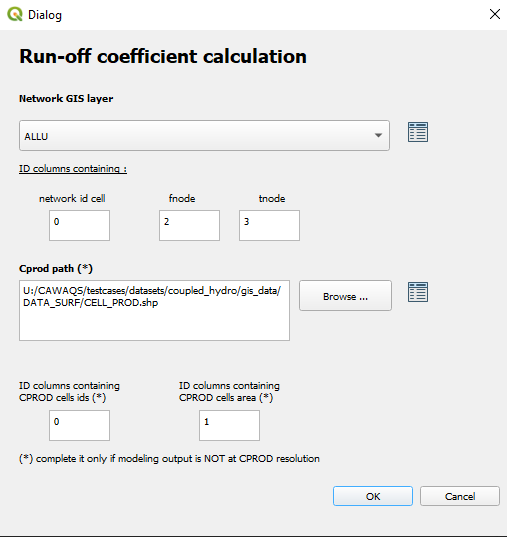
\includegraphics[width=0.5\linewidth]{
        2_application_user_guide/fig/DialogRunOffCalclulation.png
    }
    \caption{Boîte de dialogue de calcul du coefficient de ruissellement.}
    \label{fig-DialogRunoffCoeff}
\end{figure}

Cette boîte de dialogue prend en entrée la résolution du schéma hydrologique de surface à l'échelle du tronçon de rivière et la résolution de surface \cawaqs~des mailles de production (bassins versants élémentaires ou \script{Cprod}). Pour la première, le numéro de colonne contenant les identifiants de tronçons, \script{Fnode} et \script{Tnode} doivent être spécifiés. Pour la seconde, les identifiants des champs contenant l'identifiant de la maille de production et l'aire de la maille.\\

Si la résolution de surface définie dans la configuration \cwv~est déjà celle des mailles de production, il ne sera pas nécessaire de renseigner la partie inférieure de la boîte de dialogue.

Deux nouvelles résolutions (\textit{shapefiles}) seront renvoyées par la boîte de dialogue et ajoutées au projet SIG courant :
\begin{itemize}
    \item \gui{CATCH} qui contient les bassins versants drainés par chaque station de mesure ;

    \item \gui{CATCH\_SURF}, produit de l'intersection entre la résolution de surface définie dans la configuration \cwv~et \gui{CATCH}. Sa table attributaire contient plusieurs champs :
        \begin{itemize}
            \item[$-$] \gui{CATCH\_ID} et \gui{CATCH\_SURF} : l'identifiant du bassin versant drainé par la station et son aire ;

            \item[$-$] \gui{ID\_OBS} : l'identifiant de la station de mesure ;

            \item[$-$] \gui{SURF\_ID} : l'aire de la maille de surface issue de la résolution de surface définie dans la configuration \cwv~;

            \item[$-$] \gui{SURF\_SURF} : son aire ;

            \item[$-$] \gui{INTER\_ID} : l'identifiant de la maille d'intersection ;

            \item[$-$] \gui{INTER\_SURF} : l'aire d'intersection.
        \end{itemize}
\end{itemize}

Ces résolutions sont enregistrées au format temporaire. Il revient à l'utilisateur de les enregistrer pour une réutilisation future. Si \cwv~reconnaît ces résolutions dans le projet QGIS courant, elles seront réutilisées pour le calcul des coefficients de ruissellement.\\

Ces coefficients se trouvent dans la table attributaire de la couche d'observation de débit spécifiée à l'étape de configuration. Deux nouveaux champs sont alors ajoutés : \gui{QruissSim} et \gui{QruissObs} désignant respectivement le coefficient de ruissellement simulé par \cawaqs~et celui observé aux stations de mesure.

\section{\script{Compare sim/obs} : comparaison des chroniques observées et simulées}
\label{sec-com-simobs}

Ce module de calcul permet la comparaison entre simulations et observations à travers plusieurs types de sorties :
\begin{itemize}
    \item en cliquant sur \gui{PDF printout}, un fichier \script{pdf} est généré. Les chroniques simulées et observées sont présentées avec les critères statistiques listés dans la table \ref{tab_statistical_criteria_crits_fields} ;
    \item en cliquant sur \gui{Interactiv graphics}, un format \script{html} reproduit interactivement le format de présentation des chroniques du \script{pdf} dans le navigateur par défaut ;
    \item en cliquant sur \gui{Statistical criteria}, la boîte de dialogue \gui{Statistical Criteria} (\ref{sec-critstat}) s'ouvre. Les paramètres spécifiés dans la boîte de dialogue \gui{Compare Sim-Obs} (dates, compartiment et unité de mesure des observations) sont transférés à la boîte de dialogue \gui{Statistical Criteria}.
\end{itemize}

\begin{figure}[H]
    \centering
    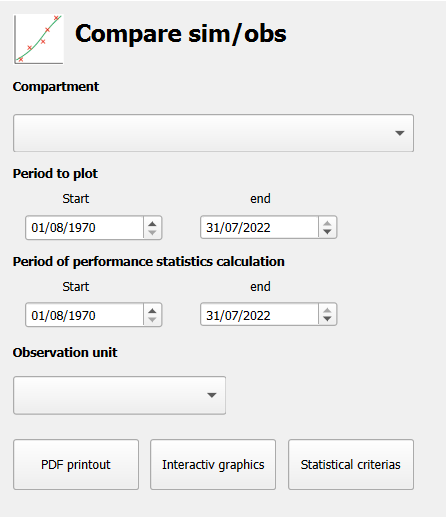
\includegraphics[width=0.45\linewidth]{
        2_application_user_guide/fig/DialogCompareSimObs.png
    }
    \caption{Fenêtre de dialogue \gui{Compare sim/obs}.}
    \label{fig-dialogCompareSimObs}
\end{figure}

Le type de compartiment (\script{AQ} = aquifère et \script{HYD} = réseau hydrographique) est à sélectionner dans la liste déroulante située dans la partie supérieure de la boîte de dialogue (\cref{fig-dialogCompareSimObs}). Les périodes d'impression des chroniques et celles de calcul des critères statistiques doivent également être spécifiées. L'unité des observations de débit, utilisée pour le traitement des simulations du compartiment \gui{HYD}, doit être précisée dans le menu déroulant \gui{Observation unit}. Elle est optionnelle pour le traitement du compartiment \gui{AQ}.\\

Un message d'information sera affiché dans l'interface QGIS à la fin de cette tâche et pointera vers le répertoire de post-traitement. Les fichiers \script{.pdf} issus de l'analyse du compartiment \script{HYD} seront nommés \gui{SIM\_OBS\_HYD.pdf} par défaut. Ceux issus de l'analyse du compartiment aquifère seront nommés \gui{SIM\_OBS\_AQ.pdf}. Chaque page de ce document correspond à une station de mesure.

\section{\script{Spatial Map} : cartographie spatiale des variables hydrologiques}
\label{sec-spatial-map}

Cet outil spatialise le bilan hydrique de surface au format \script{.shp}. Le bilan peut être produit à une fréquence annuelle, mensuelle ou journalière (à préciser dans le champ \script{frequence}). L'agrégation temporelle peut être réalisée par moyenne, somme, maximum ou minimum (à préciser dans le champ \script{agregator}).


\begin{figure}[H]
    \centering
    \begin{subfigure}
        [b]{0.48\linewidth}
        \centering
        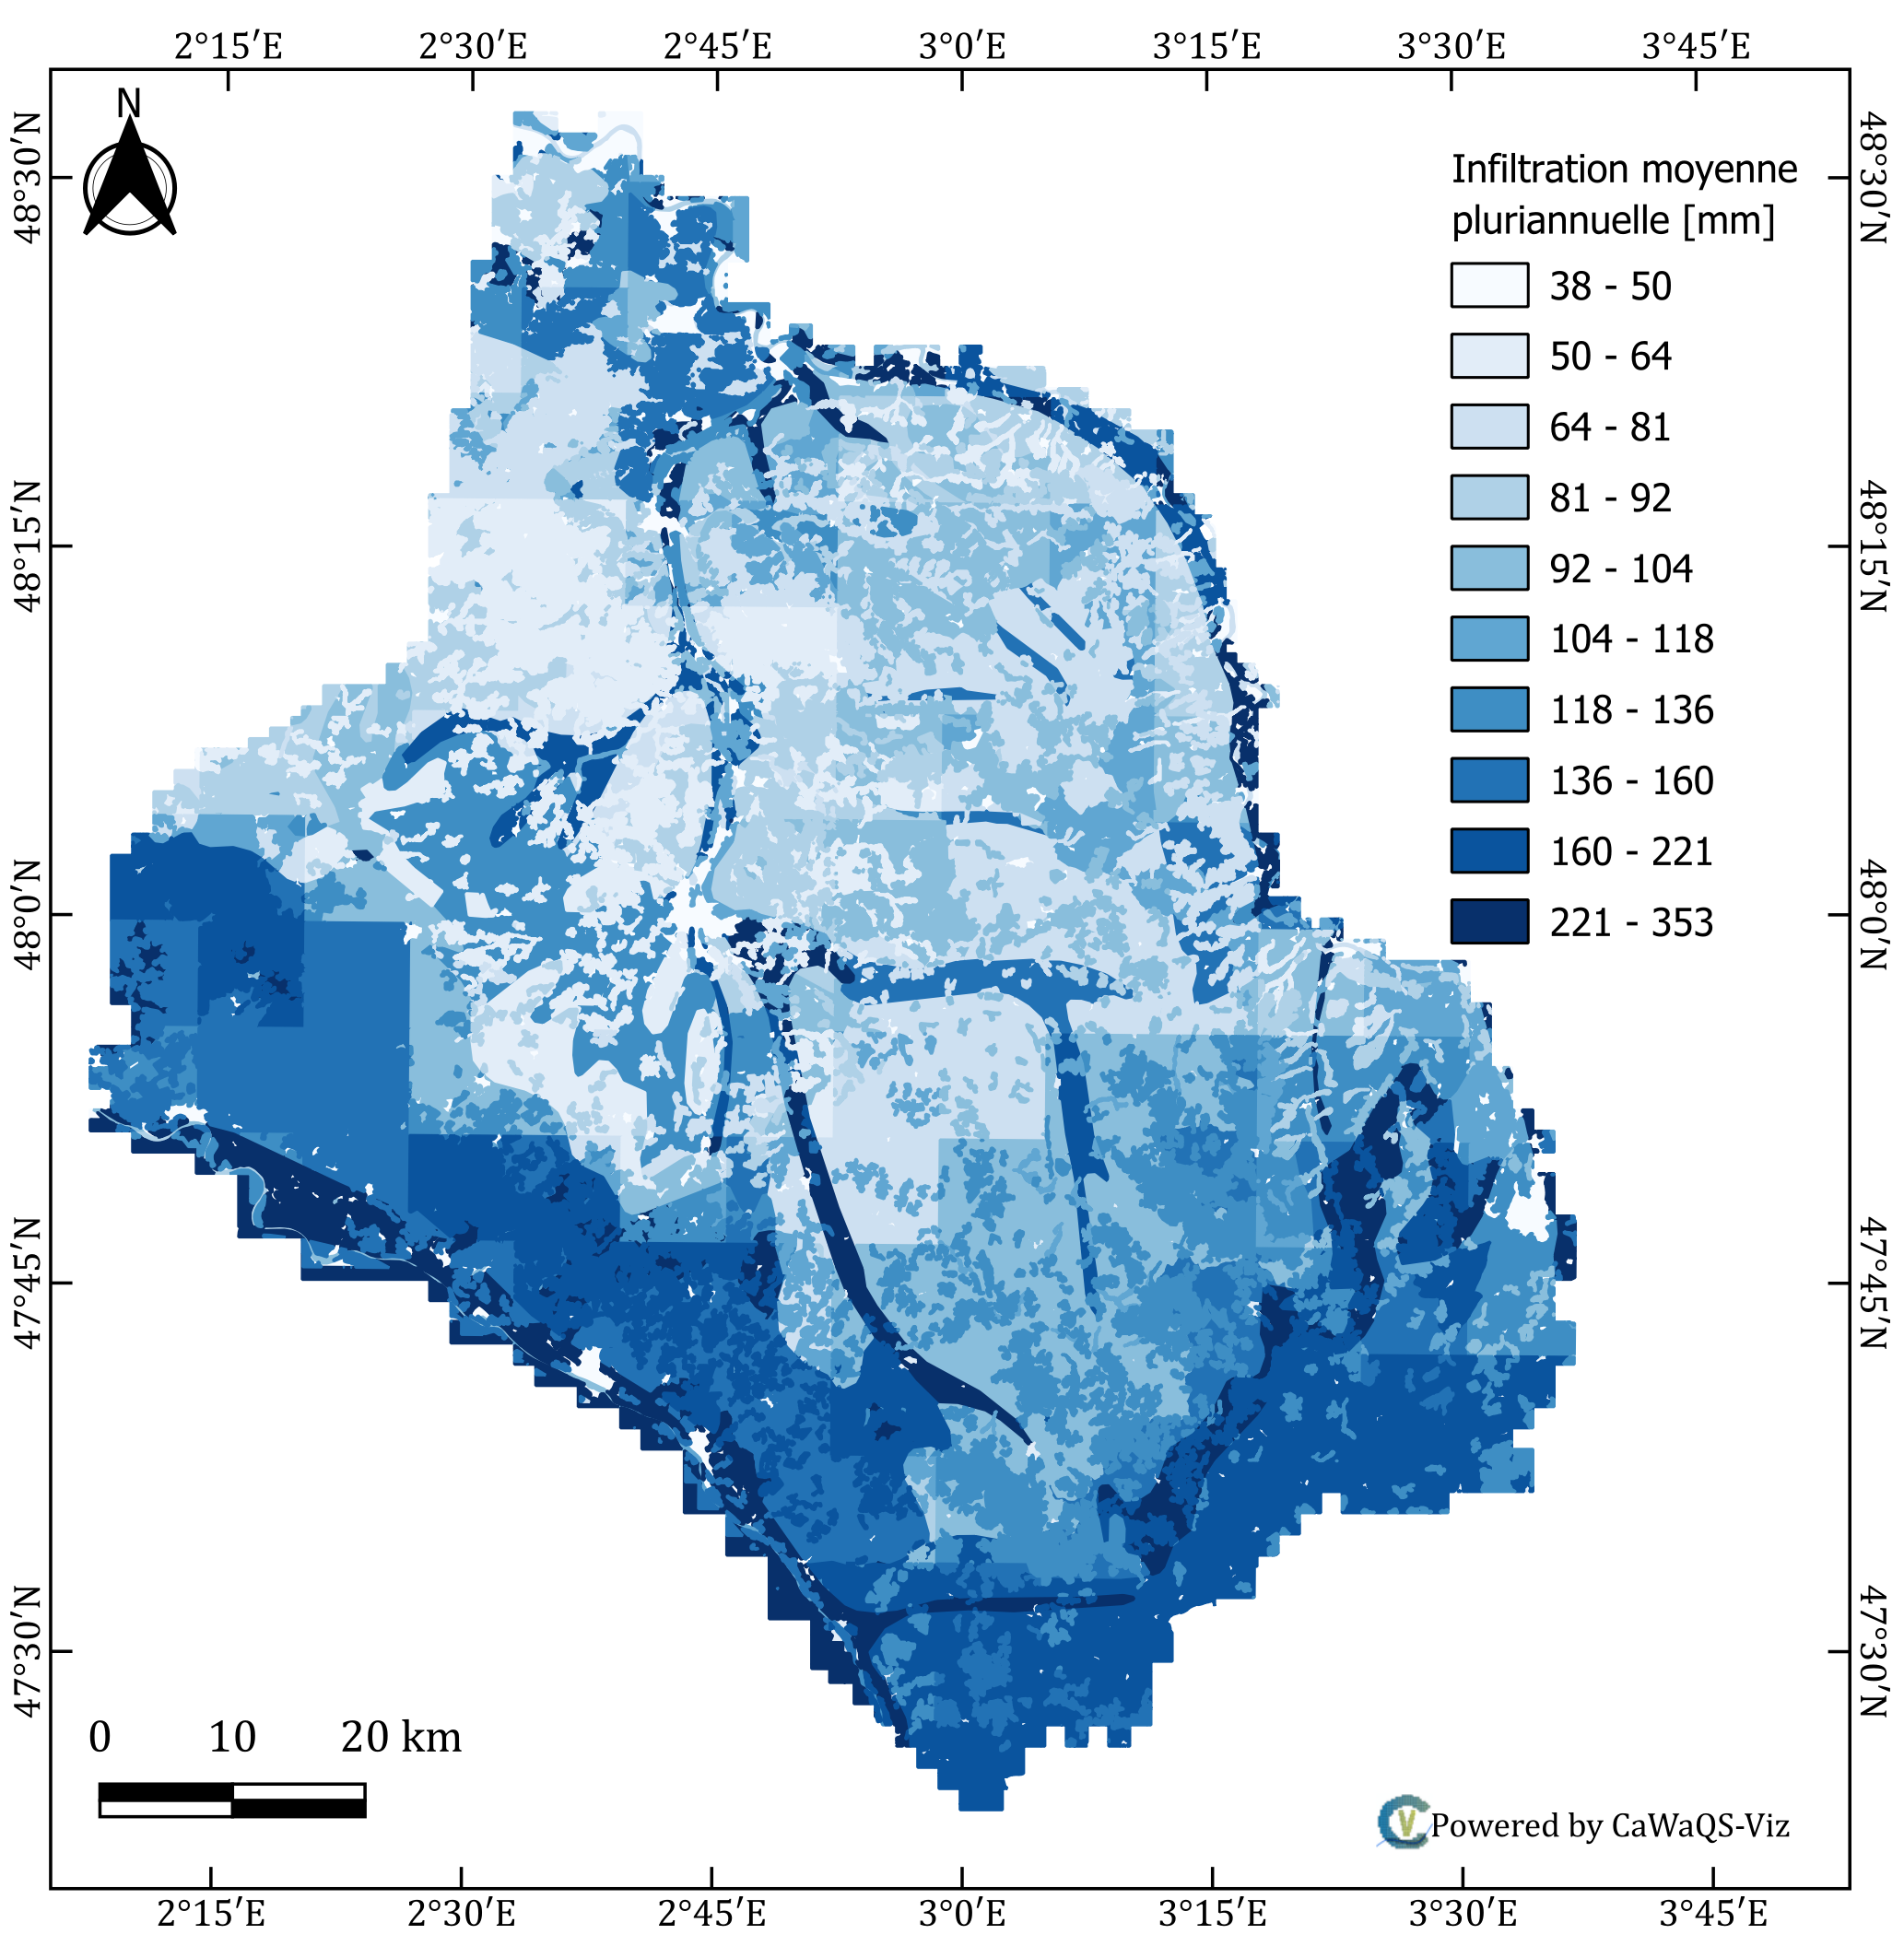
\includegraphics[width=\linewidth]{3_features/fig/OutputSpatialMap.png}
        \caption{}
        \label{fig-outSpatialMap-surf}
    \end{subfigure}
    \begin{subfigure}
        [b]{0.45\linewidth}
        \centering
        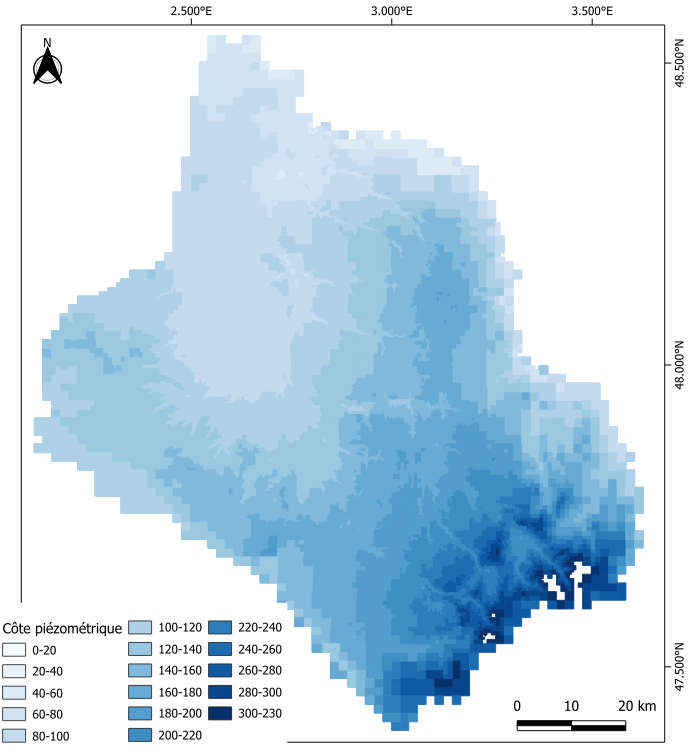
\includegraphics[width=\linewidth]{3_features/fig/Cote_piezo.png}
        \caption{}
        \label{fig-outSpatialMap-sout}
    \end{subfigure}
    \caption{Spatialisation du flux d'infiltration moyen interannuel [$mm$] (a) et de la piézométrie [$mNGF$] (b) simulés à l'échelle de l'hydrosystème du Loing}
    \label{fig:two_figures}
\end{figure}

Les valeurs prises par la variable hydrologique à spatialiser sont contenues dans la table attributaire de la résolution \script{.shp} de sortie. La table a pour colonnes les identifiants d'années pour une agrégation annuelle, les identifiants de mois pour une agrégation mensuelle et enfin la date pour une sortie au pas de temps journalier. Une agrégation pluriannuelle en moyenne est également possible en cochant la case \script{Pluriannual}, établissant ainsi un bilan pluriannuel ou pluriannuel mensuel.

\begin{itemize}
    \item \script{WATBAL} : les variables précipitation, ETR, ruissellement et infiltration (\ref{fig-outSpatialMap-surf}) ;

    \item \script{AQ} : les charges hydrauliques (\ref{fig-outSpatialMap-sout}), visualisables soit sur une couche de maillage aquifère donnée, soit sur les mailles aquifères affleurantes (maillage unique, créé par \cwv).\\
\end{itemize}

Les variables du compartiment \script{WATBAL} sont exprimées en \mmj~ou \mman~selon le mode d'agrégation choisi. Les variables du compartiment \script{AQ} sont exprimées en mètres.

\section{\script{Budget Bar Plot} : visualisation du bilan hydrologique}
\label{sec-bufget-barplot}

Les bilans hydrologiques simulés peuvent être visualisés depuis cette boîte de dialogue. Ils sont construits conformément à la période spécifiée. Le champ \script{Frequences} précise le pas de temps de calcul du bilan hydrique (pluriannuel, annuel, mensuel ou journalier), tandis que \script{agregator} précise l'agrégateur temporel (moyenne, somme, maximum, minimum). Le bilan hydrique est agrégé spatialement par une moyenne des variables hydrologiques sur l'ensemble des mailles de surface.

À l'exécution de cette boîte de dialogue, une page \script{HTML} s'ouvre dans votre navigateur et affiche un graphique interactif du bilan hydrologique. Une image statique (cf. Fig. \ref{fig-budget-barplot}) de ce même graphique est enregistrée dans le répertoire de post-traitement, dans un sous-dossier \script{../BUDGET} du répertoire de post-traitement.

\begin{figure*}[htb]
    \centering
    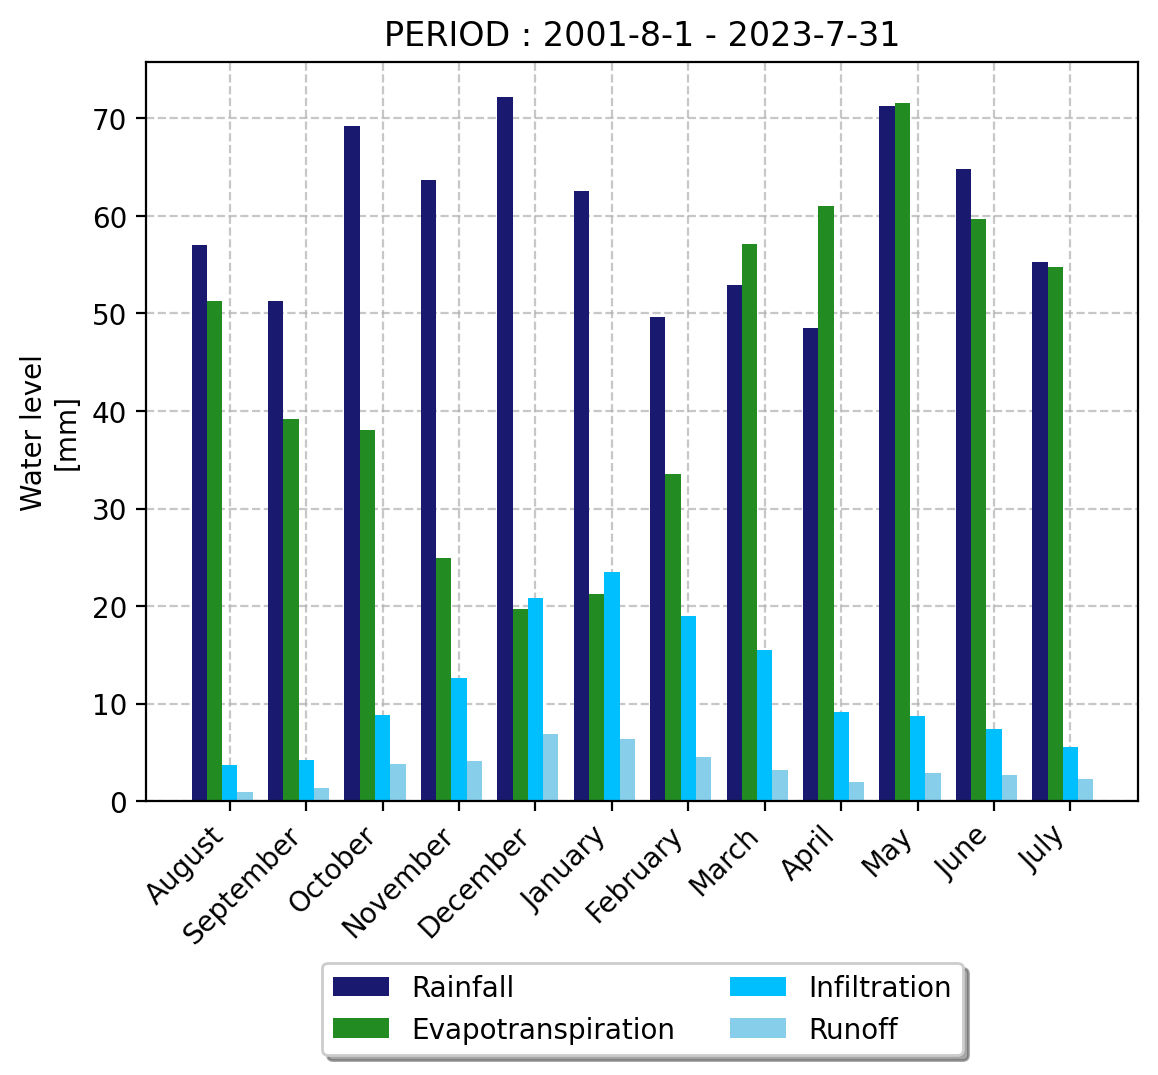
\includegraphics[width=0.55\linewidth]{
        3_features/fig/BUDGET_2001-8-12023-7-31Pluriannual_Sum.png
    }
    \caption{Exemple de sortie graphique du bilan hydrologique pluriannuel mensuel simulé}
    \label{fig-budget-barplot}
\end{figure*}

\newpage
\section{\script{Hydological Regime} : visualisation du régime hydrologique}
\label{sec-regime-hydro}

Les régimes hydrologiques simulés de l'hydrosystème sont construits depuis la boîte de dialogue \gui{Hydrological Regime} (cf. Figure \ref{fig-dialogHydroRegime}). Les régimes hydrologiques sont calculés sur la période spécifiée dans les champs de saisie \gui{Start} et \gui{end}. La variable à analyser est à préciser dans le menu déroulant \gui{Hydrological variable to plot}. Le type de sortie est choisi par l'utilisateur en cochant la case \gui{static plots (PNG)} pour des sorties graphiques sous forme d'images individuelles pour chaque point de mesure, \gui{static plots (PDF)} pour une sortie PDF compilant les régimes hydrologiques de tous les points de mesure, et enfin \gui{interractives plots} pour une sortie dans le navigateur par défaut sous forme de graphiques interactifs (\ref{fig-output-regime-hydrologique}). Une boîte de dialogue alerte l'utilisateur lorsque le module de calcul a terminé son exécution.\\

\begin{figure}[h]
    \centering
    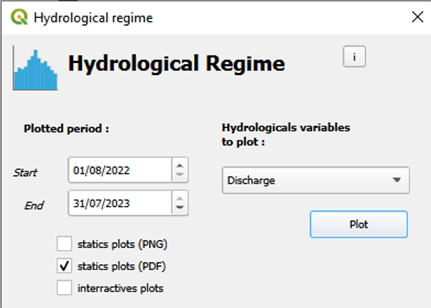
\includegraphics[width=0.5\linewidth]{
        3_features/fig/DialogHydrologicalREgime.png
    }
    \caption{Boîte de dialogue \gui{Hydrological Regime} pour le calcul des régimes hydrologiques pluriannuels mensuels.}
    \label{fig-dialogHydroRegime}
\end{figure}


\begin{figure*}[htb]
    \centering
    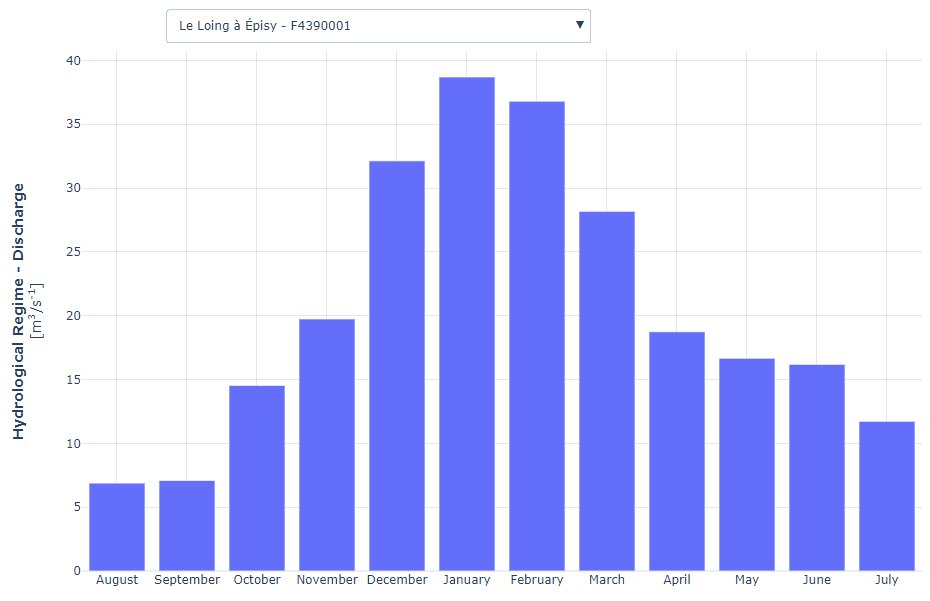
\includegraphics[width=0.5\linewidth]{
        3_features/fig/Output_regime_hydrologique.png
    }
    \caption{Exemple de sortie graphique du régime hydrologique pluriannuel mensuel simulé}
    \label{fig-output-regime-hydrologique}
\end{figure*}

\newpage
\section{\script{Extract Data from a sub area} : extraction des résultats dans un polygone}
\label{sec-extract-area}

La boîte de dialogue \gui{Extract Data from a Sub Area} (\cref{fig-dialogMask}) permet d'extraire les résultats de simulation sur une zone définie. Cette zone peut être spécifiée soit comme un polygone issu d'un \texttt{QgsVectorLayer} chargé dans le projet, soit comme un shapefile importé depuis un répertoire.

\begin{figure}[H]
    \centering
    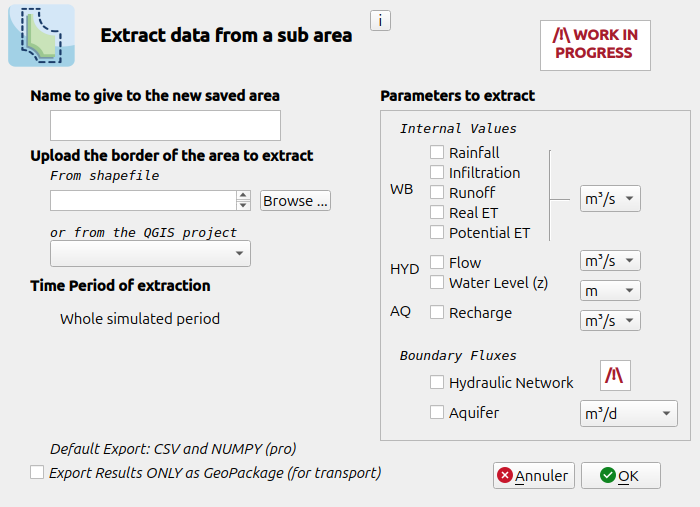
\includegraphics[width=0.5\linewidth]{
        3_features/fig/DialogMask.png
    }
    \caption{Boîte de dialogue \gui{Extract Data from a Sub Area}.}
    \label{fig-dialogMask}
\end{figure}

Deux familles de variables peuvent être extraites, chacune pilotée par son propre jeu de cases à cocher et produisant son propre ensemble de sorties : les \emph{valeurs internes} (\cref{sec-extract-internal}), c.-à-d.\ les variables simulées des compartiments \script{WATBAL}, \script{HYD} et \script{AQ} à l'intérieur du polygone, et les \emph{valeurs aux limites} (\cref{sec-extract-boundary}), c.-à-d.\ les flux traversant la frontière du polygone. Les deux familles dépendent d'une case à cocher \gui{GeoPackage} indépendante qui bascule l'ensemble du format de sortie.

\subsection{Paramètres}
\label{sec-extract-params}
Depuis la boîte de dialogue, les paramètres suivants peuvent être spécifiés pour l'extraction :
\begin{itemize}
    \item le nom du nouveau fichier d'extraction (également utilisé comme nom du dossier créé dans \texttt{PostProcessing/DATA\_EXTRACTED/}) ;
    \item le polygone d'extraction : soit un shapefile, soit un \texttt{QgsVectorLayer} présent dans le projet ;
    \item les paramètres à extraire (cases à cocher) ;
    \item l'unité de mesure, choisie dans la liste déroulante à côté de chaque paramètre (voir \cref{sec-extract-units}) ;
    \item si le format de sortie doit être un GeoPackage ou l'organisation par défaut en fichiers séparés (\cref{sec-extract-outputs}).
\end{itemize}

\subsection{Sorties}
\label{sec-extract-outputs}
Pour chaque extraction, des fichiers de résultats et des \texttt{QgsVectorLayer} sont produits. Les fichiers sont enregistrés dans le répertoire de sortie défini dans les paramètres d'analyse principaux, sous \texttt{PostProcessing/DATA\_EXTRACTED/<Extraction\_Name>}, qui contient les sous-dossiers suivants :
\begin{itemize}
    \item \textbf{CONFIG/} : fichiers de configuration pour rejouer les simulations WIP ;
    \item \textbf{OUTPUTS/} : fichiers CSV ou GeoPackage contenant les résultats ;
    \item \textbf{TEMP/} : fichiers NumPy utilisés pour rejouer les analyses.
\end{itemize}

La case à cocher \gui{GeoPackage} n'\emph{ajoute} pas de fichier, elle \emph{remplace} les fichiers séparés. Les deux modes sont mutuellement exclusifs :
\begin{itemize}
    \item \textbf{Décochée (par défaut)} : un CSV par paramètre coché dans \texttt{OUTPUTS/} et un binaire \script{.npy} par paramètre dans \texttt{TEMP/} (plus un CSV de total sur le polygone par paramètre lorsque la pondération est activée). Aucun GeoPackage n'est écrit.
    \item \textbf{Cochée} : un unique GeoPackage dans \texttt{OUTPUTS/} et rien d'autre --- ni CSV, ni \script{.npy}.
\end{itemize}

\subsection{Unités}
\label{sec-extract-units}
Chaque paramètre porte sa propre unité, choisie dans la liste déroulante à côté de sa case à cocher. Les flux \script{WATBAL}, la \gui{Recharge} \script{AQ} et le \gui{Flow} \script{HYD} sont volumiques (\texttt{m\textsuperscript{3}/s} ou \texttt{m\textsuperscript{3}/d}) ; la \gui{Water Height} \script{HYD} est une longueur (\texttt{m} ou \texttt{cm}) et n'est donc pas soumise à la conversion volumique par jour. Les flux souterrains (aux limites) \script{AQ} disposent de leur propre liste déroulante d'unités, décrite en \cref{sec-extract-boundary}.

\subsection{Paramètres --- valeurs internes}
\label{sec-extract-internal}
Les variables suivantes peuvent être extraites pour la surface (compartiment \script{WATBAL} de \cawaqs) :
\begin{itemize}
    \item \gui{Rainfall} ;
    \item \gui{Real EvapoTranspiration (ET)} ;
    \item \gui{Infiltration} ;
    \item \gui{Runoff} ;
    \item \gui{Potential EvapoTranspiration (ET)}.
\end{itemize}
Pour le réseau hydrographique (\script{HYD}) :
\begin{itemize}
    \item \gui{Flow} ;
    \item \gui{Water Height} ;
\end{itemize}
Pour l'aquifère (\script{AQ}) :
\begin{itemize}
    \item \gui{Recharge}.
\end{itemize}

\subsubsection{Le GeoPackage des valeurs internes}
\label{sec-extract-internal-gpkg}
Lorsque la case \gui{GeoPackage} est cochée, tous les compartiments cochés sont regroupés dans un unique fichier, \texttt{<area>\_InternalValues\_<years>.gpkg}, écrit dans \texttt{OUTPUTS/}. Il contient :
\begin{itemize}
    \item une couche vectorielle \texttt{cells\_<compartment>} par maillage (par ex.\ \texttt{cells\_WATBAL}, \texttt{cells\_AQ}, \texttt{cells\_HYD}) portant la géométrie masquée --- les tronçons \script{HYD} sont découpés à la frontière du polygone ;
    \item une table \texttt{daily\_values} comportant une ligne par tuple (compartiment, maille, date, paramètre) ; elle est jointe à une couche de maillage sur la paire (\texttt{compartment}, \texttt{cell\_id}) ;
    \item une table \texttt{provenance} comportant une ligne par compartiment ;
    \item une table \texttt{polygon\_total\_<compartment>\_<param>} par paramètre, lorsque la pondération est activée.
\end{itemize}

\subsection{Paramètres --- valeurs aux limites}
\label{sec-extract-boundary}
\begin{itemize}
    \item flux souterrains (horizontaux) de l'\gui{Aquifer} : les flux traversant les faces verticales des mailles aquifères situées sur la frontière du polygone ;
    \item \gui{Hydraulic network} WIP : débit des tronçons traversant les limites du masque.
\end{itemize}

\subsubsection{Convention d'unité et de signe}
La case à cocher \gui{Subsurface flows} possède sa propre liste déroulante d'unités, offrant deux options qui diffèrent par leur \emph{nature}, et pas seulement par leur échelle :
\begin{itemize}
    \item \texttt{m\textsuperscript{3}/d} (par défaut) : un \textbf{débit} journalier (le \texttt{m\textsuperscript{3}/s} brut multiplié par 86\,400), donnant une valeur par jour ;
    \item \texttt{m\textsuperscript{3}/month} : le \textbf{volume} total réel (\texttt{m\textsuperscript{3}}) ayant traversé chaque limite au cours de chaque mois calendaire. L'axe temporel est ré-échantillonné à une ligne par mois, chaque valeur étant la somme, sur les jours de ce mois, des \texttt{m\textsuperscript{3}/s} $\times$ 86\,400 journaliers. Les longueurs réelles des mois (28, 29, 30 ou 31 jours) sont respectées.
\end{itemize}

\alertinfo{En mode \texttt{m\textsuperscript{3}/month}, un premier ou dernier mois partiel ne totalise \textbf{que ses jours simulés}. Un premier ou dernier mois dont le volume paraît faible comparé à ses voisins est donc correct, et non une erreur.}

La convention de signe accompagne les données --- dans la ligne d'en-tête du CSV et dans la table \texttt{provenance} du GeoPackage : \textbf{une valeur positive signifie un flux entrant dans la maille}.

\subsubsection{Mode par défaut : le CSV des flux de faces}
Lorsque la case \gui{GeoPackage} est décochée, les flux aux limites sont écrits dans un CSV de flux de faces séparé. Les faces sont nommées selon la convention \texttt{nCell(ID\_ABS)\_direction\_unit}, par exemple \texttt{3323\_west\_m3d}. C'est le \textbf{seul} mode qui expose le détail \emph{brut} par face, c.-à-d.\ la valeur propre de chaque face prise séparément.

\subsubsection{Mode GeoPackage : le GeoPackage des limites AQ}
\label{sec-extract-boundary-gpkg}
Le GeoPackage des limites AQ est exclusif de la même manière que celui des valeurs internes : lorsque la case est cochée, un unique \texttt{<area>\_AqBoundary\_<years>.gpkg} est écrit \emph{à la place} du CSV de flux de faces séparé. Il contient :
\begin{itemize}
    \item une couche de géométrie \texttt{cells\_AQ\_layer<id>} par couche aquifère ;
    \item une table de valeurs --- \texttt{daily\_values} en mode \texttt{m\textsuperscript{3}/d}, \texttt{monthly\_values} en mode volume total \texttt{m\textsuperscript{3}/month}.
\end{itemize}

\begin{figure}[H]
    \centering
    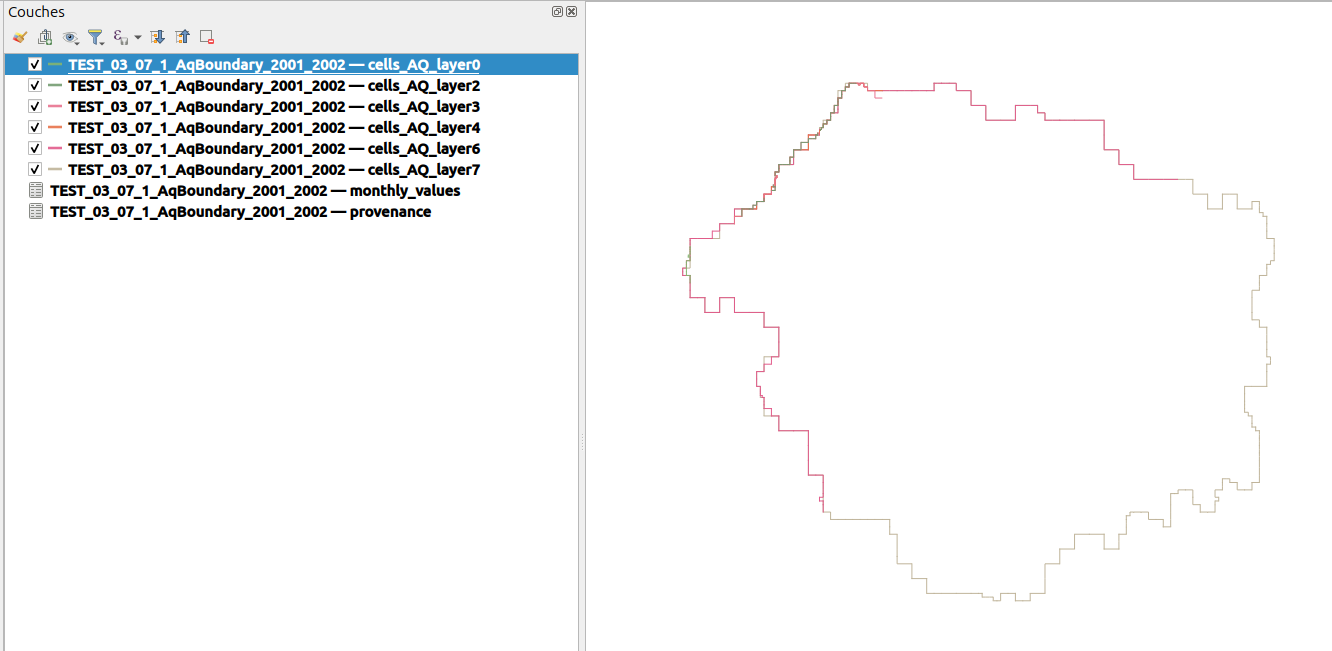
\includegraphics[width=0.5\linewidth]{
        3_features/fig/AQ_boundary_geopackage.png
    }
    \caption{\gui{AQ boundary geopackage}.}
    \label{fig-AQ-boundary-geopackage}
\end{figure}

Les couches de géométrie comme la table de valeurs portent une colonne \texttt{faces} : la liste, séparée par des virgules, des directions cardinales que chaque maille de bordure touche, par exemple \texttt{'north,west'}. Chaque ligne reste \textbf{une série nette par maille} ; la colonne \texttt{faces} indique simplement quelles directions y ont contribué. La colonne \texttt{faces} apparaît aussi dans la table attributaire de la couche de bordures QGIS enregistrée dans le projet, indépendamment du mode GeoPackage.

\paragraph{Colonnes de structure par face.} À l'intérieur du fichier GeoPackage uniquement, sept colonnes supplémentaires répartissent ce résumé sur des champs interrogeables. Elles apparaissent à la fois sur les couches de géométrie \texttt{cells\_AQ\_layer<id>} et sur la table de valeurs, mais \textbf{pas} sur la couche de bordures QGIS enregistrée, qui ne conserve que \texttt{faces}.
\begin{itemize}
    \item \texttt{n\_faces} : nombre de côtés cardinaux que borde la maille (1 à 3) ;
    \item \texttt{face1\_orient}/\texttt{face1\_outid} \dots{} \texttt{face3\_orient}/\texttt{face3\_outid} : deux colonnes par emplacement de face.
\end{itemize}
\texttt{faceN\_orient} est la $N$-ième direction bordée ; les emplacements au-delà de \texttt{n\_faces} sont laissés vides. \texttt{faceN\_outid} n'est renseigné \textbf{que} lorsque le flux de cette face provient de la maille extérieure --- le cas \emph{coarse-inside}, où la valeur reportée provient des voisines extérieures plus petites, dont les identifiants sont alors joints par des virgules dans le champ. Il reste vide pour une lecture normale de la face propre.
